\subsection{Multithreaded Cluster and Track Finding Algorithms} \label{ssec:val_multithreaded_ctf}
Considering that the nature of the changes done to the code in this version relate purely to using additional threads to compute results and do not reduce the CPU time, but only the throughput.
It's worth noting that the style of figures that's been used up until now is no longer appropriate, so another is used.

The total time for the DCHB and DCTB engines are compared by running only the multithreaded cluster finding algorithm (version $1.4.\text{a}$), only the multithreaded track finding (version $1.4.\text{b}$), and using both algorithms together (version $1.4$) to get the final total engine time for all the work in this document.
These improvements can be seen in Figure \ref{fig:engines_times-1_4}.

    \begin{figure}[ht]
        \centering
        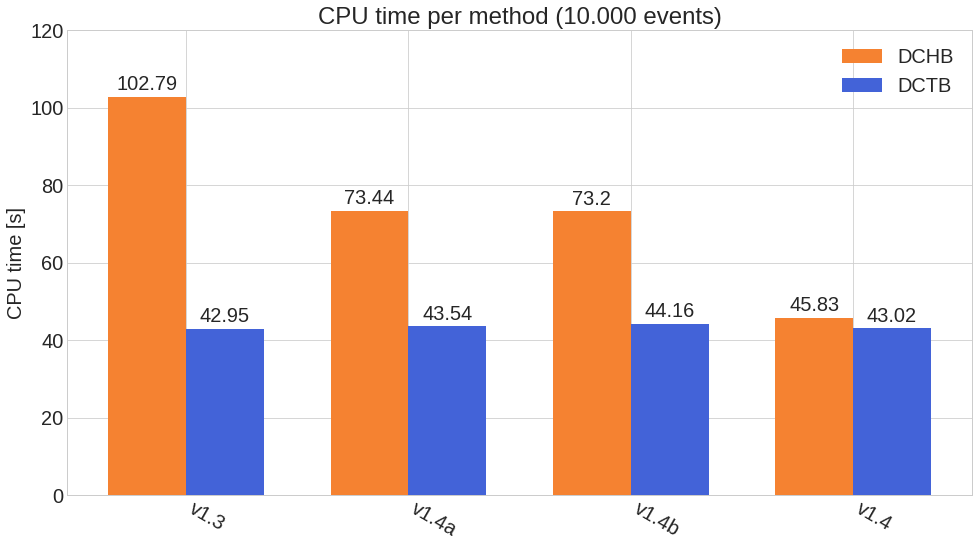
\includegraphics[scale=0.44]{engine_times/mctf_contrast}
        \caption{\label{fig:engines_times-1_4} DCHB and DCTB final CPU times, version $1.4$ compared with $1.3$. Versions $1.4.\text{a}$ and $1.4.\text{b}$ represent only the multithreaded cluster finding and track finding algorithms respectively, while version $1.4$ denotes both together.}
    \end{figure}

\newpage

It's very important to keep in mind that, unlike the other figures, the engine times improvement seen in this figure are not necessarily representative of the actual improvement that will be seen at JLab if and when the changes are implemented.
This is because, as mentioned previously, the hardware used to run the performance tests was a personal computer, and not the cluster where the final implementation will be used.
In its real context, the effectiveness of this version will depend in part on the number of free cores available while running the program, and thus the results obtained will fluctuate depending on this variable.